\documentclass[12pt,a4paper]{article}

\usepackage[T1]{fontenc}
\usepackage[utf8]{inputenc}
\usepackage[brazil]{babel}
\usepackage{lmodern}
\usepackage[a4paper,margin=2.5cm]{geometry}
\usepackage{graphicx}
\usepackage{booktabs}
\usepackage{array}
\usepackage{float}
\usepackage{hyperref}
\usepackage{xcolor}
\usepackage{setspace}

\hypersetup{
    colorlinks=true,
    linkcolor=black,
    urlcolor=blue
}

\graphicspath{{figures/}}
\setstretch{1.12}
\setlength{\parindent}{1.25cm}
\setlength{\parskip}{0.35em}

\newcommand{\AuthorName}{Raphael Damasceno Rocha de Moraes}
\newcommand{\AuthorEmail}{raphael.damasceno@unifesp.br}

\newcommand{\VisualCorrect}{59}
\newcommand{\VisualPartial}{22}
\newcommand{\VisualIncorrect}{19}

\begin{document}

\begin{titlepage}
    \centering
    {\large Universidade Federal de Sao Paulo\par}
    \vspace{1.2cm}
    {\Large\bfseries Laboratorio 02: Deteccao de Pratos com Transformada de Hough\par}
    \vspace{2.0cm}
    {\large \AuthorName\par}
    \vspace{0.2cm}
    {\normalsize \texttt{\AuthorEmail}\par}
    \vfill
    {\large Relatorio tecnico\par}
    \vspace{0.4cm}
    {\large \today\par}
\end{titlepage}

\section{Objetivo}

Este trabalho teve como objetivo detectar automaticamente pratos em imagens de refeicoes por meio da Transformada de Hough para circulos. A ideia central foi receber um conjunto de imagens coloridas, aplicar um pre-processamento simples e, em seguida, localizar o prato principal de cada cena. Nao ha componente de aprendizado de maquina aqui. O problema e tratado como um experimento classico de visao computacional, com ajuste de parametros e avaliacao visual dos resultados.

O enunciado pedia uma implementacao em C++ com OpenCV, uso das 100 imagens fornecidas e geracao de saidas visuais para apoiar a analise. Esse fluxo foi seguido integralmente. Um ponto importante e que a deteccao de circulos nao foi delegada para uma funcao pronta da biblioteca. A acumulacao de votos foi implementada no proprio codigo, com OpenCV sendo usado apenas nas etapas auxiliares de leitura, pre-processamento, gradiente, bordas e desenho das saidas.

\section{Base de dados}

Foi utilizada a base fornecida para o laboratorio, composta por 100 imagens JPEG. As imagens apresentam pratos em condicoes variadas: iluminacao irregular, pratos parcialmente cortados, utensilios sobre a comida, fundos com estampas, bordas com baixo contraste e, em varios casos, refeicoes que ocupam grande parte da area interna do prato. Isso deixa o problema menos trivial do que uma deteccao circular limpa em fundo uniforme.

Nao foi feita separacao entre treino e teste, porque o enunciado nao exige isso e a avaliacao e visual. Assim, as 100 imagens foram processadas em todos os experimentos.

\section{Implementacao}

O codigo foi organizado em modulos simples. O arquivo \texttt{main.cpp} coordena a execucao geral, os parametros ficam em \texttt{config.*}, a logica da deteccao esta em \texttt{plate\_detector.*} e a parte de leitura/escrita de arquivos esta em \texttt{io\_utils.*}. A implementacao foi feita em C++17 com OpenCV.

O pipeline usado no experimento ficou assim:

\begin{enumerate}
    \item leitura das imagens do diretorio de entrada;
    \item conversao para tons de cinza;
    \item aplicacao de filtro da mediana e filtro gaussiano;
    \item uso opcional de CLAHE em alguns testes;
    \item deteccao de circulos com uma implementacao propria da Transformada de Hough;
    \item atribuicao de um \emph{score} aos circulos candidatos;
    \item escolha do prato principal com base nesse score;
    \item gravacao das imagens anotadas e dos arquivos CSV.
\end{enumerate}

Na implementacao da Hough, primeiro foram obtidas as bordas com Canny e os gradientes com Sobel. Depois disso, para cada pixel de borda e para cada raio dentro da faixa testada, foram gerados votos para possiveis centros ao longo da direcao normal do gradiente, nos dois sentidos. Os votos foram acumulados em uma grade de centros, e os picos locais acima de um limiar passaram por uma verificacao adicional de suporte na circunferencia. Assim, o metodo nao depende de \texttt{cv::HoughCircles}; a etapa principal foi escrita no proprio projeto.

Um segundo ponto importante foi nao aceitar simplesmente o pico bruto mais forte da acumuladora. Como algumas imagens geram muitos candidatos, foi usada uma funcao de pontuacao que combina suporte obtido na Hough, raio maior, proximidade do centro da imagem e penalizacao para circulos cortados na borda. Isso ajudou a priorizar o prato principal sem tornar a regra excessivamente complexa.

\section{Pre-processamento}

Os pre-processamentos usados foram intencionais e relativamente conservadores. Primeiro foi feita a conversao para escala de cinza, o que ja reduz bastante a variacao cromatica da cena e deixa a deteccao mais ligada a contorno e contraste. Em seguida, foi aplicado filtro da mediana para reduzir ruido pontual e pequenas texturas. Depois disso, foi usado filtro gaussiano para suavizar bordas muito quebradas antes da Hough.

Tambem foi testado CLAHE em um dos presets. Na pratica, ele ajudou em imagens mais apagadas ou com contraste baixo na borda do prato, mas em algumas cenas trouxe mais estruturas concorrentes e aumentou a quantidade de candidatos secundarios. Ou seja, foi util em parte da base, mas nao resolveu o problema de forma uniforme.

Pelo comportamento observado, os filtros de mediana e gaussiano foram os mais estaveis ao longo da base. O CLAHE foi mais situacional. Diferentemente de uma chamada pronta da biblioteca, aqui a borda por Canny fez parte do proprio pipeline da Hough implementada manualmente, junto com os gradientes usados para orientar os votos.

\section{Parametros testados}

Foram definidos tres conjuntos principais de parametros. Isso facilitou a comparacao sem transformar o experimento em uma busca exaustiva muito grande.

\begin{table}[H]
    \centering
    \caption{Presets avaliados no experimento}
    \begin{tabular}{>{\raggedright\arraybackslash}p{2.5cm}ccccccccc}
        \toprule
        Preset & dp & minDist & Canny & Acc & minR & maxR & Mediana & Gauss & CLAHE \\
        \midrule
        balanced  & 1.2 & 90  & 120 & 36 & 90  & 240 & 5 & 7 / 1.5 & nao \\
        sensitive & 1.1 & 75  & 100 & 28 & 80  & 250 & 5 & 9 / 1.8 & sim \\
        strict    & 1.3 & 100 & 140 & 42 & 100 & 220 & 5 & 7 / 1.2 & nao \\
        \bottomrule
    \end{tabular}
\end{table}

O preset \texttt{balanced} foi pensado como ponto de partida mais neutro. O preset \texttt{sensitive} ficou mais permissivo, com limiares menores e uso de CLAHE, tentando recuperar pratos que apareciam de forma parcial ou com bordas menos nitidas. Ja o preset \texttt{strict} foi mais rigido e, por isso mesmo, acabou rejeitando varios casos onde o prato estava presente mas nao apresentava uma borda circular forte o suficiente.

\section{Resultados obtidos}

O programa foi executado sobre as 100 imagens com o modo \texttt{--sweep}, o que gerou uma pasta de resultados para cada preset. As saidas incluem imagens anotadas, um arquivo \texttt{detections.csv} com os circulos escolhidos e um \texttt{classification\_template.csv} para preenchimento manual da avaliacao visual.

\begin{table}[H]
    \centering
    \caption{Resumo automatico das deteccoes por preset}
    \begin{tabular}{lccc}
        \toprule
        Preset & Imagens processadas & Deteccoes & Sem deteccao \\
        \midrule
        balanced  & 100 & 99  & 1 \\
        sensitive & 100 & 100 & 0 \\
        strict    & 100 & 97  & 3 \\
        \bottomrule
    \end{tabular}
\end{table}

Esses numeros, sozinhos, nao bastam para fechar a avaliacao, porque detectar algum circulo nao significa necessariamente detectar o prato principal de forma boa. Mesmo assim, eles ja mostram o comportamento geral. Depois da calibracao da Hough manual, a cobertura ficou alta nos tres presets, com destaque para o \texttt{sensitive}, que encontrou ao menos um candidato em todas as imagens. O \texttt{balanced} ficou mais equilibrado em varios casos, enquanto o \texttt{strict} continuou mais suscetivel a perder pratos em situacoes de contraste ruim ou geometria parcial.

Considerando a inspecao feita durante os testes, o preset \texttt{sensitive} pareceu o mais interessante para usar como configuracao principal do experimento, principalmente porque ele recupera imagens onde os presets mais conservadores ainda podem falhar. Ainda assim, isso nao significa que ele seja visualmente melhor em todos os casos. Em algumas imagens ele superdetecta a cena e produz muito ruido de candidatos secundarios.

\section{Exemplos qualitativos}

\subsection{Casos em que o metodo funcionou bem}

Para a avaliacao visual final, foi adotado o preset \texttt{balanced}. As Figuras~\ref{fig:correct0}, \ref{fig:correct13} e \ref{fig:correct18} mostram exemplos classificados como corretos. Nesses casos, mesmo com textura interna, comida cobrindo grande parte do prato ou leve inclinacao da cena, o circulo escolhido acompanha de forma convincente a borda principal.

\begin{figure}[H]
    \centering
    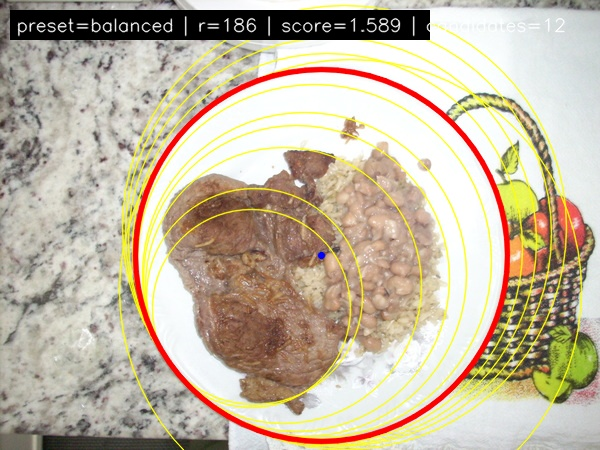
\includegraphics[width=0.72\textwidth]{correct_0.jpg}
    \caption{Exemplo classificado como correto no preset \texttt{balanced} (imagem 0).}
    \label{fig:correct0}
\end{figure}

\begin{figure}[H]
    \centering
    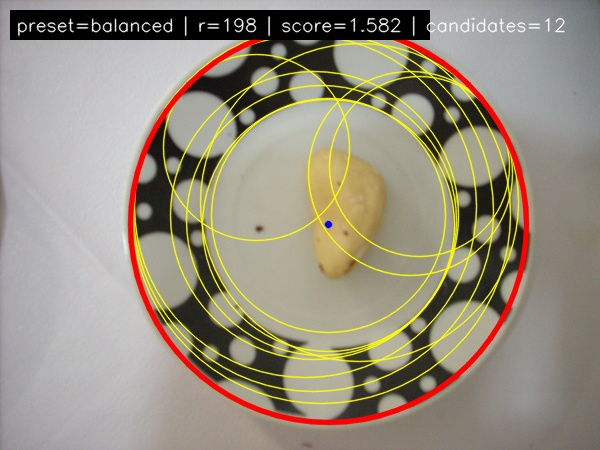
\includegraphics[width=0.72\textwidth]{correct_13.jpg}
    \caption{Outro caso de boa localizacao do prato principal (imagem 13).}
    \label{fig:correct13}
\end{figure}

\begin{figure}[H]
    \centering
    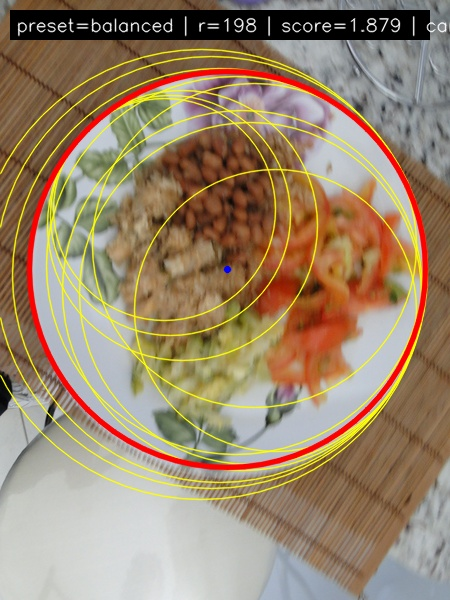
\includegraphics[width=0.72\textwidth]{correct_18.jpg}
    \caption{Deteccao correta em uma imagem com prato inclinado e conteudo interno mais irregular (imagem 18).}
    \label{fig:correct18}
\end{figure}

\subsection{Casos parcialmente satisfatorios}

Ha imagens em que o prato principal e localizado, mas com algumas ressalvas. O raio pode ficar um pouco maior ou menor do que o ideal, a borda pode ser inferida apenas de forma aproximada, ou a regiao escolhida fica deslocada em relacao ao prato principal. As Figuras~\ref{fig:partial100}, \ref{fig:partial57} e \ref{fig:partial63} mostram esse comportamento. Em todos esses casos, a deteccao ainda tem utilidade visual, mas nao considero o resultado plenamente satisfatorio.

\begin{figure}[H]
    \centering
    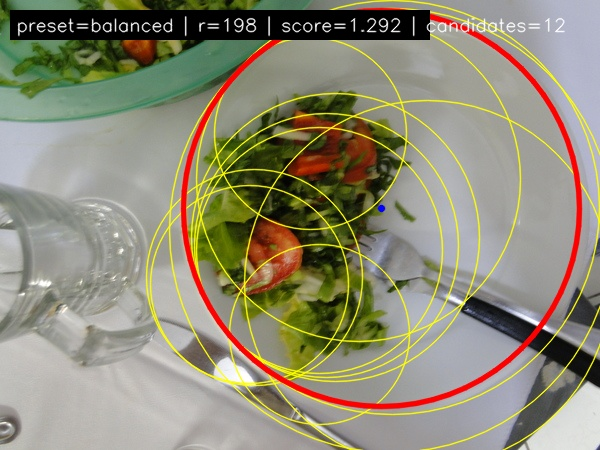
\includegraphics[width=0.72\textwidth]{partial_100.jpg}
    \caption{Deteccao parcial em prato parcialmente fora do enquadramento (imagem 100).}
    \label{fig:partial100}
\end{figure}

\begin{figure}[H]
    \centering
    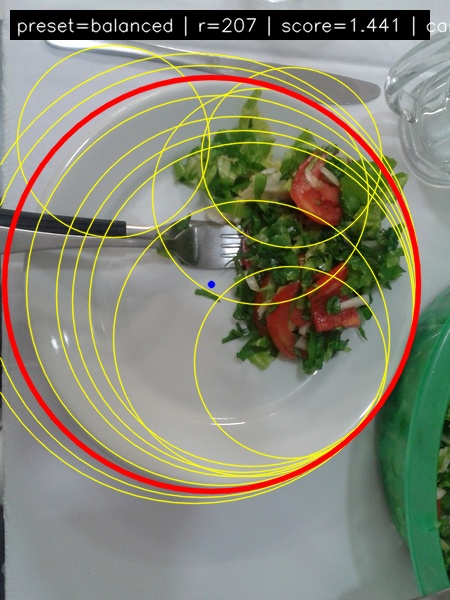
\includegraphics[width=0.72\textwidth]{partial_57.jpg}
    \caption{Caso parcial em que o prato e encontrado, mas com ajuste visual apenas aproximado (imagem 57).}
    \label{fig:partial57}
\end{figure}

\begin{figure}[H]
    \centering
    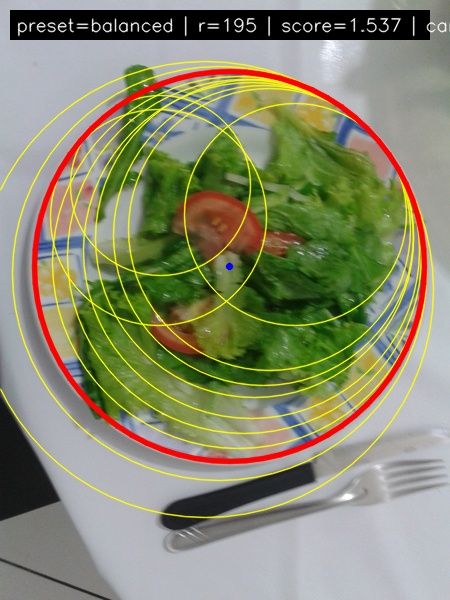
\includegraphics[width=0.72\textwidth]{partial_63.jpg}
    \caption{Exemplo parcial com borda razoavelmente localizada, embora ainda com ambiguidade no encaixe do circulo (imagem 63).}
    \label{fig:partial63}
\end{figure}

\subsection{Casos de falha}

As falhas aparecem de modos diferentes. Em alguns casos o circulo escolhido recai sobre uma regiao interna do prato e nao sobre sua borda externa. Em outros, a posicao final fica bastante deslocada, o que compromete a interpretacao. As Figuras~\ref{fig:incorrect21}, \ref{fig:incorrect58} e \ref{fig:incorrect83} mostram exemplos que, na avaliacao final, foram classificados como incorretos.

\begin{figure}[H]
    \centering
    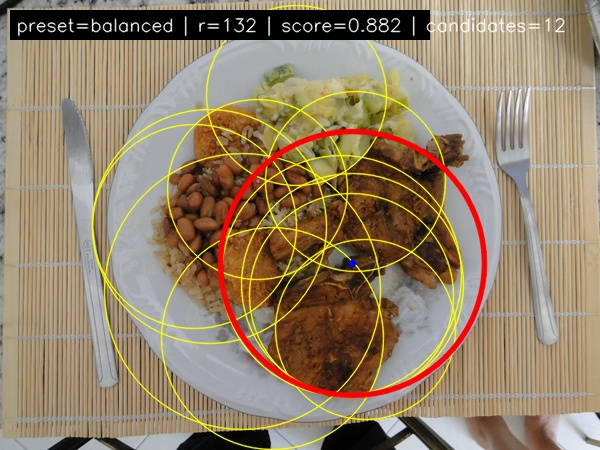
\includegraphics[width=0.72\textwidth]{incorrect_21.jpg}
    \caption{Falha em que o circulo escolhido recai sobre uma regiao interna do prato, sem acompanhar a borda principal (imagem 21).}
    \label{fig:incorrect21}
\end{figure}

\begin{figure}[H]
    \centering
    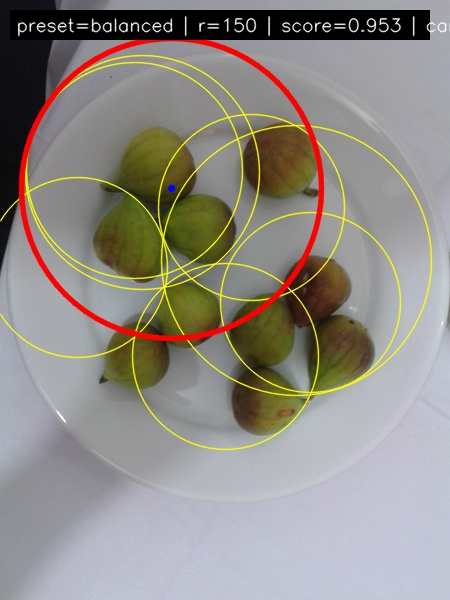
\includegraphics[width=0.72\textwidth]{incorrect_58.jpg}
    \caption{Exemplo incorreto com deteccao deslocada para apenas uma parte do prato (imagem 58).}
    \label{fig:incorrect58}
\end{figure}

\begin{figure}[H]
    \centering
    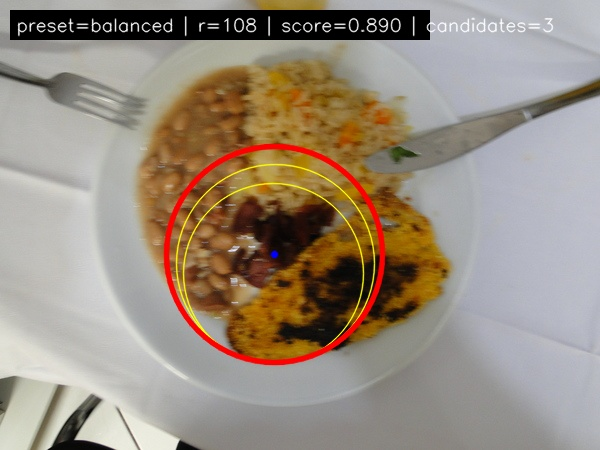
\includegraphics[width=0.72\textwidth]{incorrect_83.jpg}
    \caption{Falha em cena mais complexa, com encaixe ruim do circulo escolhido em relacao ao prato principal (imagem 83).}
    \label{fig:incorrect83}
\end{figure}

\section{Tabela obrigatoria da avaliacao visual}

O enunciado pede a contagem final em tres categorias visuais. A classificacao manual foi feita sobre as imagens anotadas do preset \texttt{balanced}, e os totais obtidos aparecem na tabela abaixo.

\begin{table}[H]
    \centering
    \caption{Contagem final por categoria visual}
    \begin{tabular}{lc}
        \toprule
        Categoria & Quantidade \\
        \midrule
        Detectado corretamente & \VisualCorrect \\
        Detectado parcialmente & \VisualPartial \\
        Nao detectado ou detectado incorretamente & \VisualIncorrect \\
        \midrule
        Total & 100 \\
        \bottomrule
    \end{tabular}
\end{table}

\section{Dificuldades encontradas}

A maior dificuldade nao foi chamar a funcao da Hough em si, mas fazer com que ela respondesse de forma razoavel em uma base heterogenea. Em imagens com pratos bem contrastados e quase frontais, a deteccao funciona de maneira direta. Ja nas imagens com utensilios fortes sobre a borda, estampa de mesa muito marcada, baixa iluminacao ou prato parcialmente fora do enquadramento, a resposta oscila bastante. Em varias delas, pequenos ajustes no limiar mudavam o resultado de forma perceptivel.

Outra dificuldade foi escolher um unico conjunto de parametros para os 100 casos. Um preset mais conservador gera menos falsos positivos, mas deixa passar pratos reais. Um preset mais sensivel melhora a cobertura, so que traz mais candidatos concorrentes. Na pratica, o experimento acabou mostrando bem esse compromisso. Como a Hough foi implementada manualmente, tambem foi preciso calibrar a propria regra de votacao, o espacamento entre raios, o limiar da acumuladora e a verificacao de suporte na circunferencia.

\section{Conclusao}

O objetivo do laboratorio foi atendido. Foi implementada uma solucao em C++ com OpenCV para detectar pratos por meio da Transformada de Hough, com pre-processamento simples, comparacao entre diferentes configuracoes e geracao de imagens de saida para avaliacao visual. A parte central de deteccao foi implementada no proprio codigo, sem usar uma rotina pronta da biblioteca para detectar circulos. O programa processa toda a base, salva os resultados e organiza os dados para o relatorio.

Entre os conjuntos testados, o preset \texttt{sensitive} se destacou pela cobertura completa da base, embora nem sempre com a deteccao mais limpa. O preset \texttt{balanced} produziu algumas imagens visualmente mais organizadas, mas perdeu pratos que ainda eram detectaveis por uma configuracao mais permissiva. O preset \texttt{strict}, por sua vez, se mostrou util como contraste experimental, mas restritivo demais para ser a melhor opcao geral.

De forma geral, a experiencia confirma um ponto conhecido em visao computacional classica: a Transformada de Hough pode funcionar bem para objetos aproximadamente circulares, mas a qualidade final depende bastante do pre-processamento e, principalmente, da calibracao dos parametros frente a variacoes reais da base.

\end{document}
